The \textit{Analyser} class in charge of managing all phases in the pipeline, in other words, it sends to each module the required input in order to obtain is output. Besides, as it has been explained in Section \ref{section:typomod} where the typographic correction module was presented, it asks the user the necessary information for the purpose of detecting and correcting, if it is required, the found typographic errors. In addition to it, as we can see in Figure \ref{fig:umlanalyser}, this class is able to store information in the database and extract it through the \textit{SessionTypoError} class.

\begin{figure}[h]
	\centering%
	\centerline{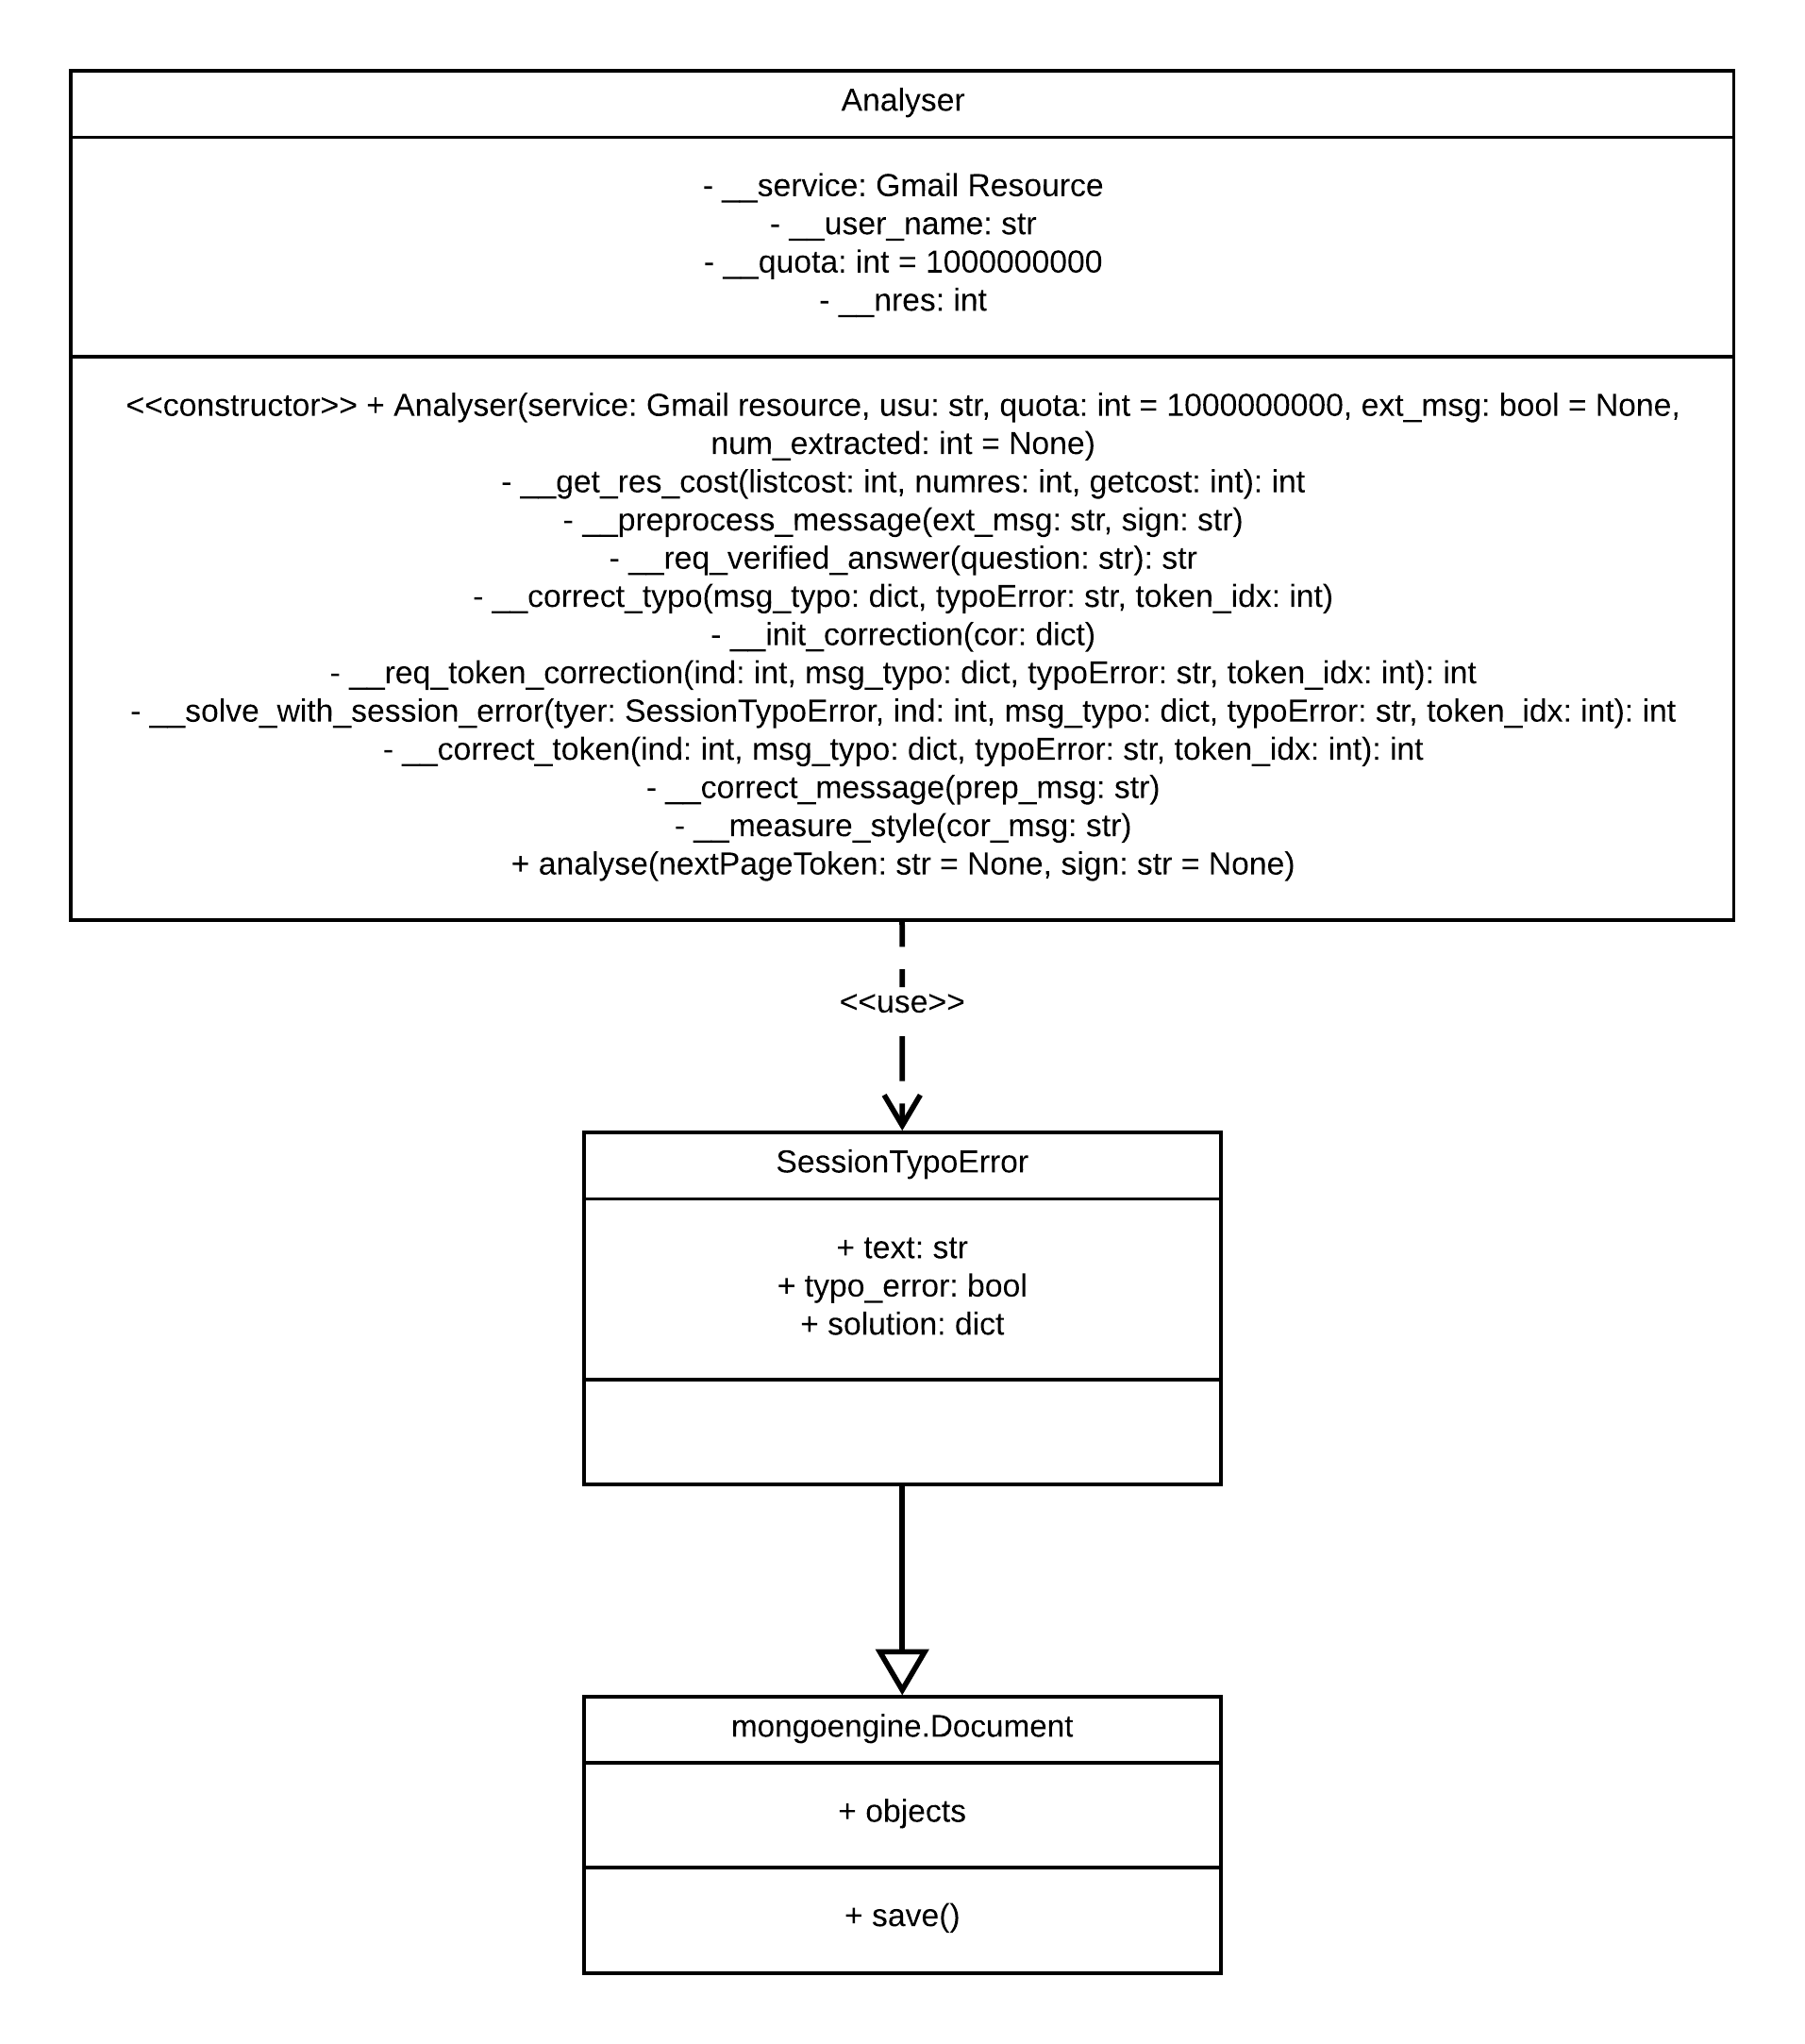
\includegraphics[width=0.6\paperwidth]{Imagenes/Bitmap/Analyser/analyserUML.png}}%
	\caption{UML class diagram of the Analyser}%
	\label{fig:umlanalyser}
\end{figure}

The \textit{Analyser}'s class constructor has an special interest in this system, due to it chooses the type of extraction that is going to be executed: a message extraction or a thread extraction. With the purpose of making this choice, the \textit{get} method of the labels resource is invoked in order to obtain the value of the fields \textit{messagesTotal} and \textit{threadsTotal} of the \textit{SENT} label structure (see Section \ref{sssect:labres}). With this values tha \textit{Analyser} is able to calculate the quota units cost (as we see in Section \ref{section:extmod}) of each type of extraction (this task is carried out by the \textit{\_\_get\_res\_cost} method) and choose the one which minimises it. After deciding it, it gives effect to the choice by creating the corresponding object with the type of extraction (\textit{MessageExtractor} or \textit{ThreadExtractor}).

Once an \textit{Analyser} object is created, the entire system can start its execution by calling the \textit{analyse} function (the web services of the modules which represent the last three phases in the pipeline have to be running). During the execution of this method, the only module that will require the attention of the \textit{Analyser} is the typographic correction module. The rest of the packages will only need this class to provide the input messages and collect their output structures.

If the \textit{TypoCorrector} detects a typographic error, the first action that the \textit{Analyser} carries out is searching in the database if that word was previously found and corrected it. For this purpose, the \textit{SessionTypoError} stores the common typographic errors that a user made (this collection is dropped at the beginning of each execution) and how to solve it (the \textit{solution} field has the same structure as the items of the list \textit{corrections} of the structure given by the \textit{TypoCorrector}). If it is a real typographic error, the \textit{typo\_error} field will take the value \textit{True} and in the \textit{solution} dictionary the text that should replace the word is stored. If it is not, the \textit{solution} dictionary will be appended to the \textit{corrections} list and the message will go on being corrected.

In the case that this typographic error is not stored, the \textit{Analyser} will ask the user whether the message has to be discarded (this option allows the user to remove from the pipeline, for instance, e-mail written in other languages). If it is discarded, the \textit{Analyser} sends then next message ready to be corrected to the typographic correction module. If it is not discarded, the \textit{\_\_req\_token\_correction} method is invoked. This function will ask the user whether the word is a real typographic error. If it is, there are two solutions: remove the token from the text or rewrite it. Either way, at the end the user is going to answer the question: ``Do you want to save this information for this session?'' In this way the user will decide whether the solution is inserted in the collection managed by \textit{SessionTypoError} in case the same error is detected again.

If it is not a real typographic error, the user will answer some questions about the token: such as whether it is an url, an e-mail, a punctuation mark, a stop word, what its part of speech is and what its lemma is. Then, this information is appended to the \textit{corrections} list and ask the user whether this information is stored in \textit{Correction} collection for the future or in \textit{SessionTypeError} collection for this session.

Once the detected word is managed, the \textit{Analyser} resends the message to the typographic correction module in order to go on correcting it.

